\documentclass{article}
\usepackage[utf8]{inputenc}
\usepackage{amsmath}
\usepackage{amsfonts}
\usepackage{mathrsfs}
\usepackage{graphicx}
\usepackage{subcaption}
\usepackage{hyperref}
\usepackage[top=25truemm,bottom=25truemm,left=25truemm,right=25truemm]{geometry}


\title{The effect of dynamic change in parameters of a dynamic social network model }
\author{Kansuke Ikehara (Kansuke.Ikehara@colorado.edu)}

\begin{document}
\maketitle
\section*{Abstract}
In this study, I investigate how dynamic change in parameters of a dynamic social network model affects the evolution of networks in terms of their structure. The state of a network is defined as a coordinate in the state space whose axes correspond to network statistics, namely \textit{clustering coefficient} and \textit{average path length} respectively. I run the network model with different parameter settings: static, randomly changing, changing according to sine functions and changing with R$\ddot{\text{o}}$ssler equation. The resulting dynamics of a trajectory for each setting is consistent with the parameter setting: static parameters lead the network state to be in some fixed point; randomly changing parameters push the state into a specific region in the state space, moving the network state randomly in the region; sinusoidally and chaotically changing parameters let the state circulate around regions in the state space.

\section{Introduction}
The study of networks (graphs) and its applications have been a great interest across many disciplines, including biology, social science and engineering \cite{Newman:2010:NI:1809753}. The focus has been, however, mainly on the static aspect of networks, namely people only investigate a snap shot of dynamically evolving networks sampled at a certain time. Since focusing on a snap shot of a dynamic networks only captures a portion of its true nature, one needs to take the time axis into account for better understanding the underlying process.

There are some works on dynamic network processes. Barabasi and Albert proposed a dynamic growing network model called \textit{BA model}, in which each node is added to a network each time, establishing an edge between some existing node\cite{BA_Model}. The model incorporates an idea called \textit{preferential attachment}. That is, new coming node tends to prefer nodes with high degree (number of edges connected to them).

Kumar \textit{et al.} proposed a model which produces a network with similar attributes as real world online social networks \cite{Kumar:2006:SEO:1150402.1150476}. In the model, nodes (users of a social network ) are categorized as follows: 1. passive users who join the network but never involve any activity, 2. inviters who basically bring off-line social network into the online social network and 3. linkers who participate in the growth of the social network by actively connecting to other users. At each time step, a new node comes assigned to one of the node types and connects to existing nodes with different probabilities depending on its type.

However, most of the works on dynamic network models focus on the resulting network structure, such as whether the model produces power-law degree distribution, high clustering coefficient and other properties observed in the real world networks. Also as far as I know, all of them fix the parameters of a model. However, the underlying process behind the real world phenomena could change the model's parameters over the course of action. For example, following preference of a user in Twitter could change over time, which might be attributed to the changes in parameters of a human behavior model. For instance, a Twitter use's initial preference for following might by inclined to celebrities, but as time passes he/she might follow politicians, scholars, etc. And the change in model's parameters would ultimately lead the network structure to be different from the its previous state.

In this study I investigate how the \textit{state} of a network  generated from a model evolves over time and the effect of changing parameters according to some functions in the dynamics. The model I use is explained in the next section.

\section{Model}
The model used in this study is proposed by Jin \textit{et al.} in \cite{PhysRevE.64.046132}. Originally, they proposed two models which describe the growing mechanism of real world social networks, one with relatively intricate model description and the other which is much simper. I use the latter model in that it simplifies the implementation and runs faster thanks to its simplicity, yet gives the almost identical behavior as the more complicated model. The notable aspects of the model are explained in the following:
\begin{itemize}
\item A node (person) can have at most $z^*$ friends at most. This explains our cognitive limit to maintaining our friendships.
\item An edge (friendship) can disappear. In a real world social network, friendship can disappear due to conflicts and/or oblivion, as we all know.
\item A node is likely to be connected to another if there are many mutual connections. This explains an abundance of triangles in social networks.
\item the number of nodes is fixed. This condition simplifies the model and is attributed to the fact that the speed of node creation/deletion (birth/death) in social networks is much slower than edge creation/deletion.
\end{itemize}

Let $n_{p} = \frac{1}{2}N(N-1)$ be the number of pairs of vertices in the network. Let $n_{e} = \frac{1}{2}\Sigma_{i}z_{i}$ be the number of existing edges, where $z_{i}$ is the degree of a node $i$. And let $n_{m} = \frac{1}{2}\Sigma_{i}z_{i}(z_{i}-1)$ be the total number of mutual neighbors of pairs of nodes in the network. With those constants defined above and three parameters, $r_{0}$,$r_{1}$ and $\gamma$, the model process at each time is defined in three steps as follows:

\begin{enumerate}
\item Choose $n_{p}r_{0}$ pairs of nodes uniformly at random from the network. Place an edge between them if there is no edge already and neither of nodes has $z^*$ degree already. In the context of social networks, this means that a person becomes a friend with a random person.

\item Choose  $n_{m}r_{1}$ nodes at random with a probability proportional to $z_{i}(z_{i}-1)$. For each chosen node, place an edge between one pair of its neighbors. This step means that a person introduces one of his/her friends to another.

\item Choose $n_{e}\gamma$ nodes with a probability proportional to $z_{i}$. For each chosen node, pick up one of its neighbors and delete the edge between them. This step corresponds to eliminating friendship.
\end{enumerate}

Three parameters of the model, namely $r_{0}$,$r_{1}$ and $\gamma$, have different effect on the growing network structure: $r_{0}$ controls the randomness in the network, $r_{1}$ controls the density of triangles and $\gamma$ controls the frequency of edge deletion.

\section{Network Statistics}
 In order to capture the evolution of a network over time, we utilize network statistics \cite{Brandes:2005:NAM:1062400}. Network statistics is an aggregated information regarding the network structure, which is often the average of local structure. Ones that are commonly investigated and also what I use in this study are the followings:
 
 \begin{enumerate}
\item \textit{Clustering Coefficient} $CC$ is an indicator of an abundance of triangles in a network. The definition as follows:
\[
	cc = \frac{\text{number of closed triplets (triangles)}}{\text{number of connected triplets}}
\]
which can be interpreted as the probability that a connected triplet is actually a triangle. It is well known that social networks exhibit high clustering coefficient compared to other kinds of networks.

\item \textit{Average Path Length} $APL$ is, as the name implies, the average distance between pairs of nodes in the network. Calculating involves a shortest path algorithm on every pair of nodes, thus computationally hard. Since the model I have described above can produce disconnected component, \textit{APL} is calculated only on the largest connected component of the network.
\end{enumerate}

With these two network statistics, we can define the \textit{state} of a network in the state space whose $x,y$ axes correspond to $CC$ and $APL$.

\section{Experiment}
The experiment for extracting a network's state trajectory is carried out for each setting as follows: run the steps 1 and 2 defined above until $90\%$ of the $N = 250$ nodes have $z^* = 5$ degree. Parameters in this initial process are the same throughout the study ($r_{0}=0.0005$, $r_{1}=2$).
 After this initial configuration, the model proceeds to full steps and uses parameters which are either fixed or changed according to some functions.
 
 In settings of dynamic parameters, I use random function, sine function and R$\ddot{\text{o}}$ssler equation. For sine function and R$\ddot{\text{o}}$ssler equation, one needs to map a value produced by those functions to a value in a desirable range. I use the following mapping equation in order to accomplish it:
\begin{equation}
 	newval = \frac{(oldval - oldmin)*y}{x} + newmin
\end{equation}
 where, \textit{oldval} is a value produced by the original function,  \textit{oldmin} is the minimum value the original function produces,  \textit{y} is the absolute value of the desired range,  \textit{x} is the same quantity for original function and \textit{newmin} is the minimum value for the desired value range. Since the vivid change in network structure occurs only when parameters change in the order of magnitude, the desired range is log scale. That is, for example, $r \in \left[ \log10^{-5},\log10^{-1}\right]$ and $newval^* = \exp(r)$. 
 
 The model runs $3000$ times for each setting, excluding the initial configuration process.
 
\section{Results}
Fig.\ref{q1}a-d show the state space trajectories for each of the parameter setting: fixed, randomly changing, sinusoidally changing and chaotically changing parameters. 

\subsection{Fixed parameters}
In fig.\ref{q1_1}, 5 trajectories each with different fixed parameter setting show different behavior in the state space. Followings are the settings:
\[
	\texttt{normal\_1}: \texttt{r0 = 0.0005, r1 = 2, gamma = 0.005}
\]
\[
	\texttt{normal\_2}: \texttt{r0 = 0.001, r1 = 2, gamma = 0.001}
\]
\[
	\texttt{normal\_3}: \texttt{r0 = 0.0001, r1 = 2, gamma = 0.01}
\]
\[
	\texttt{normal\_4}: \texttt{r0 = 0.00001, r1 = 5, gamma = 0.01}
\]
\[
	\texttt{normal\_5}: \texttt{r0 = 0.1, r1 = 0.001, gamma = 0.1}
\]

There are overall 3 behaviors in the trajectories. The first one is evolving down- and leftward and staying there, which can be seen in \texttt{normal\_1} and \texttt{normal\_2}. The second is evolving down- and a bit rightward and converging to points in the area, as seen in \texttt{normal\_3} and \texttt{normal\_4}. The last one is quickly moving down- and leftward and reaching a fixed point (in \texttt{normal\_5}). All of these behaviors have an interpretation in terms of network structure and it is explained in the next section.

\subsection{Randomly changing parameters}
First, a random value for a parameter is generated in $\log$ scale, e.g. $r \in \left[ \log(10^{-2}), \log(10^1)\right] = \left[-4.6, 2.3\right]$, then $r$ is used for a power of an exponential $\exp(r)$, which becomes the parameter of the model. Changing parameters randomly yields distinct trajectories from the ones with fixed parameters. In fig.\ref{q1_2}, the trajectory starts around the initial configuration and moves down- and leftward. It then randomly walks around the region. 

\subsection{Sinusoidally changing parameters}
Fig.\ref{q1_3} shows the trajectories for parameters which change according to sine functions. The trajectory \texttt{sin\_1} has parameters all having  the same phase for sine functions. \texttt{sin\_2\_phase\_shift}, however, has sine functions for parameters, each of which is phase-shifted by $\frac{\pi}{2}$ to others. The effect of phase-shifting is quite obvious: the location of a periodic orbit is moved up- and rightward and the orbit is made fatter.

\subsection{Chaotically changing parameters}
In this setting, I change parameters according to R$\ddot{\text{o}}$ssler equation, whose $x,y,z$ coordinates are mapped to $r_{0},r_{1},\gamma$.
For this setting, I have run the model 20 times and average trajectories in order to filter out the noise. 

\begin{figure}[h]
\centering
\begin{subfigure}{.5\textwidth}
  \centering
  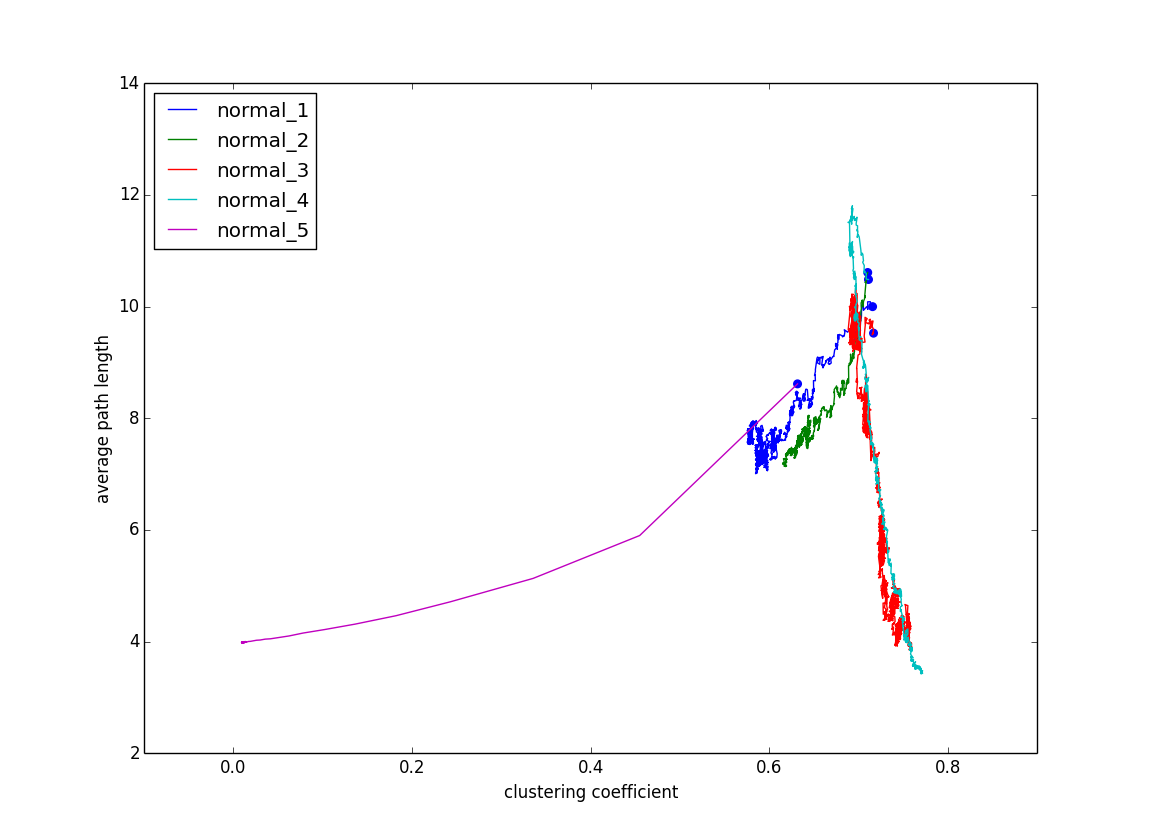
\includegraphics[height=2in]{figs/normal.png}
  \caption{normal}
  \label{q1_1}
\end{subfigure}%
\hfill
\begin{subfigure}{.5\textwidth}
  \centering
  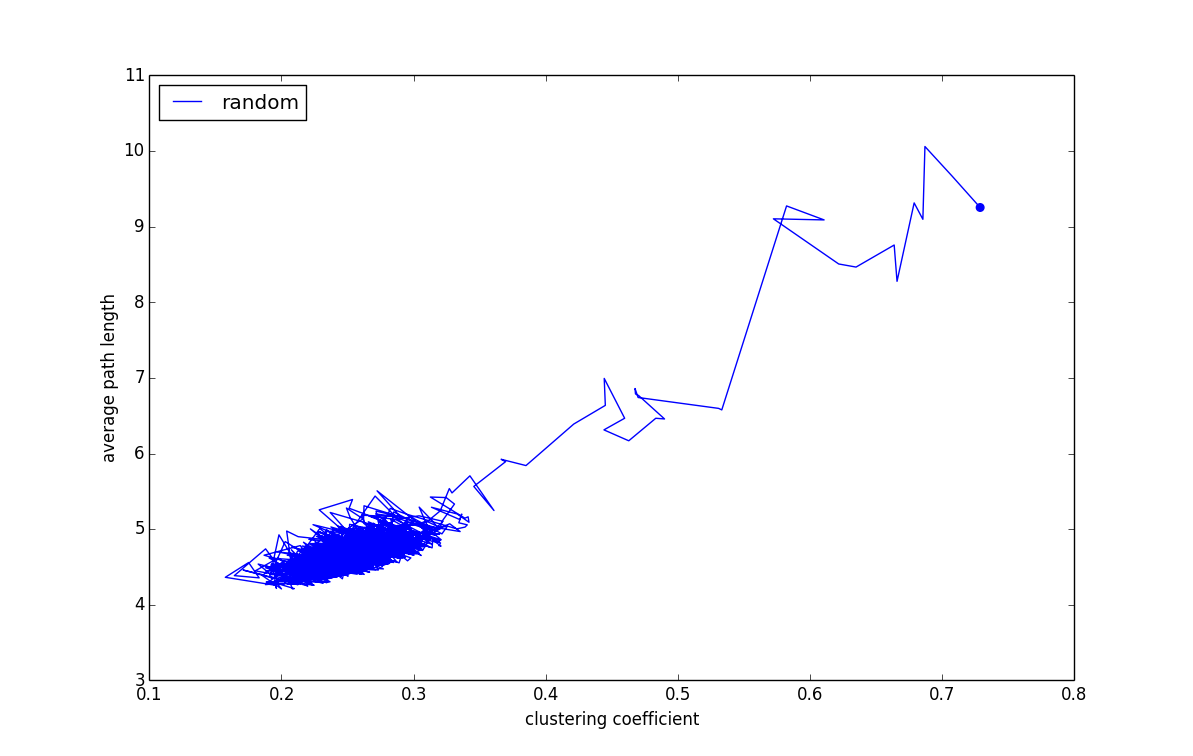
\includegraphics[height=2in]{figs/random.png}
  \caption{random}
  \label{q1_2}
\end{subfigure}%
\hfill
\begin{subfigure}{.5\textwidth}
  \centering
  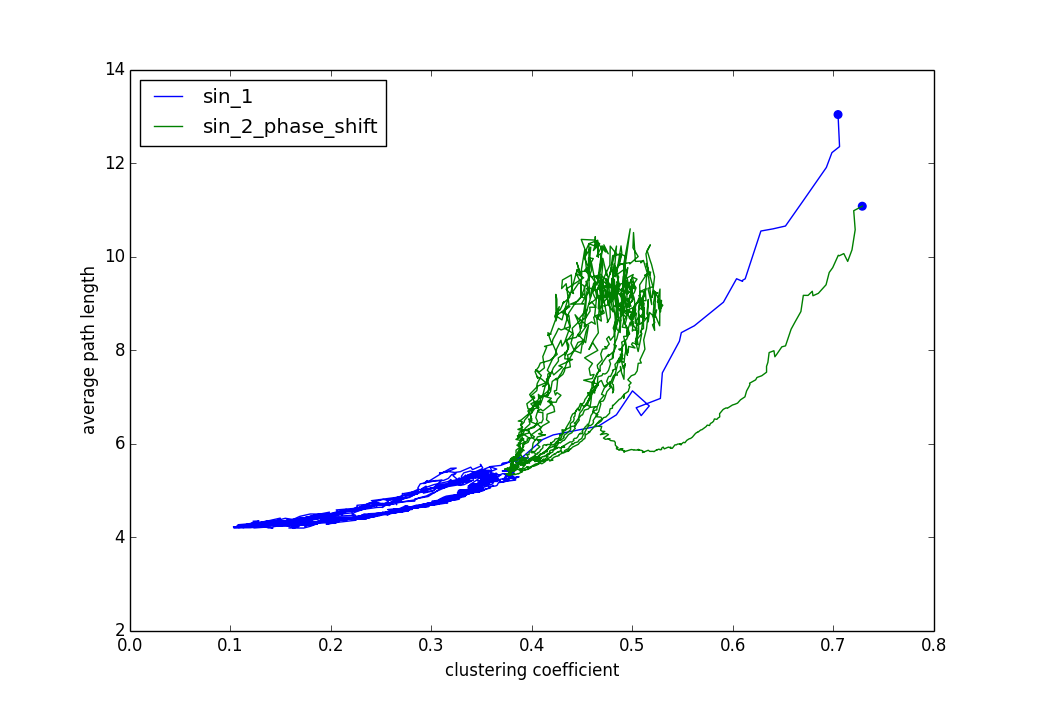
\includegraphics[height=2in]{figs/sin.png}
  \caption{sine}
  \label{q1_3}
\end{subfigure}%
\hfill
\begin{subfigure}{.5\textwidth}
  \centering
  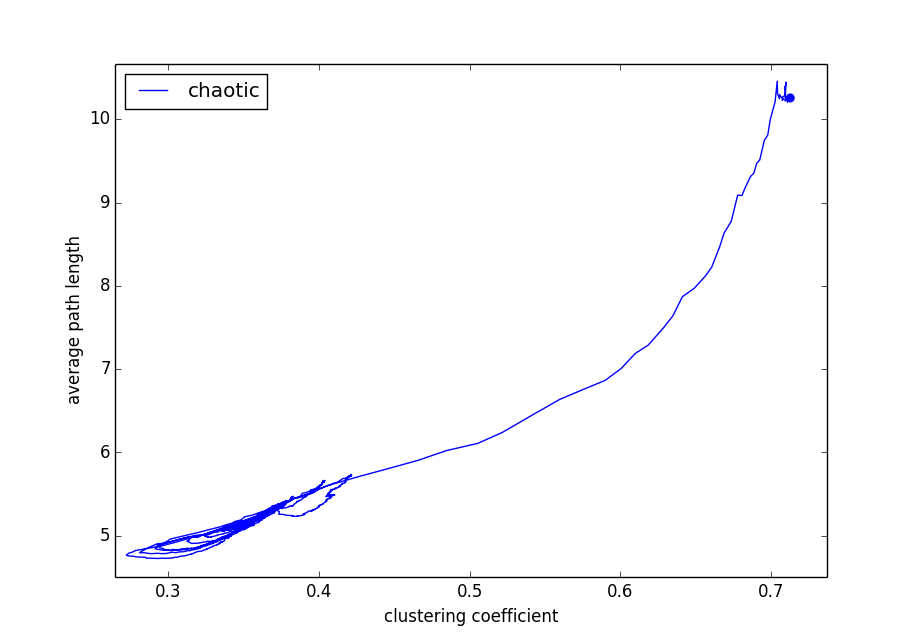
\includegraphics[height=2in]{figs/chaotic.png}
  \caption{chaotic}
  \label{q1_4}
\end{subfigure}
\caption{State-space trajectories}
\label{q1}
\end{figure}
 
 \section{Discussion}
 Fig.\ref{q2} shows how one should interpret the state in terms of network structure. The region in the bottom left corresponds to Random Network (\textit{RN}) \cite{RandomNetwork}. It is widely known that random networks have very low clustering coefficient and average path lengths. Most of the trajectories we have seen asymptotically move toward this region. On the right side of Random Network region, we see highly clustered small networks, which are usually called \textit{small-world network} (\textit{SWN}) \cite{j1998collective}. Trajectories \texttt{normal\_3} and \texttt{normal\_4} converges to be in this region. Above this region is Highly Clustered Wide Network region (\textit{HCWN}), where a network contains the number of triangles/community but the edge density between them is much sparser than those of other two network regions. 
 
 In the diagram, the evolution of trajectories correspond to shifts in the structural phase. For example, fixed parameters force networks to be converge to one of the three network type from being highly clustered and wide network. Randomly changing parameters make networks to evolve into one between Random Network and Small-World network regions and let them change randomly around the region. Sinusoidally changing them forces the network structure to be changing among \textit{RN}, \textit{SWN} and \textit{HCWN}. Chaotically changing parameters produces a similar result as one in sine function settings.
  
  The most notable point in the result is that shifting phases by $\frac{\pi}{2}$ in sine functions changes the location of a periodic orbit. This could be due to the fact that each time the most influential parameter is different. 
     
 \begin{figure}[h]
  \centering
  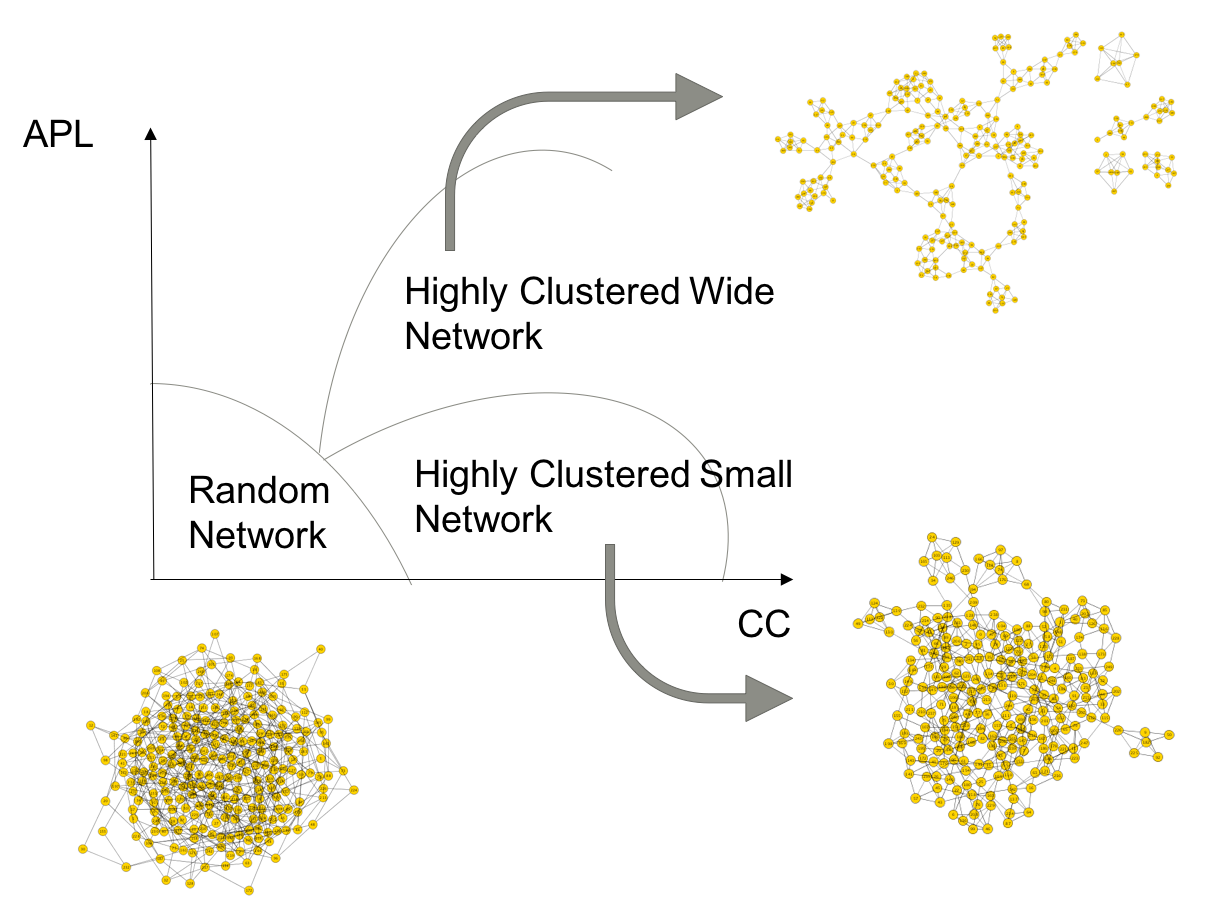
\includegraphics[width=3in]{figs/diagram.png}
  \caption{Structural interpretation for each region in the state space}
  \label{q2}
\end{figure}

\section{Conclusion}
In this study I investigate the effects of changing parameters of a model dynamically. Most of the cases, our simple intuition that networks evolve in the same way as parameters do seems to work: direct convergence to fixed points for fixed parameters, moving randomly around fixed points for randomly changing parameters, forming some sort of periodic orbits for sinusoidal parameters and chaotic parameters. However, introducing phase-shifting in sine functions yields the change in the location of a periodic orbit and its geometrical shape. This study sheds light on a new perspective in studying dynamical networks with a simple state-space approach with network statistics.

\bibliographystyle{ieeetr}
\bibliography{reference} 
\end{document}












